\section{Umsetzung}

In diesem Kapitel wird beschrieben, wie die Anforderungen praktisch
umgesetzt wurden. Zunächst wird darauf eingegangen, wie Shapes gezeichnet
werden, danach wie Spray passenden Code für Spray Web generieren kann
und zuletzt wie Spray Web Modelle validiert und persistiert.

Hier zunächst eine Bildschirmaufnahme des entgültigen Resultats
auf Abbildung \ref{fig.screenshot}.
Diese hat zur Zeit das Regelwerk für Petrinetze geladen.
Man beachte insbesondere die Ähnlichkeit zum GUI Entwurf auf Abbildung
\ref{fig.gui} die aus den Anforderungen hervorgegangen ist.

\begin{figure}[h!]
  \centering
  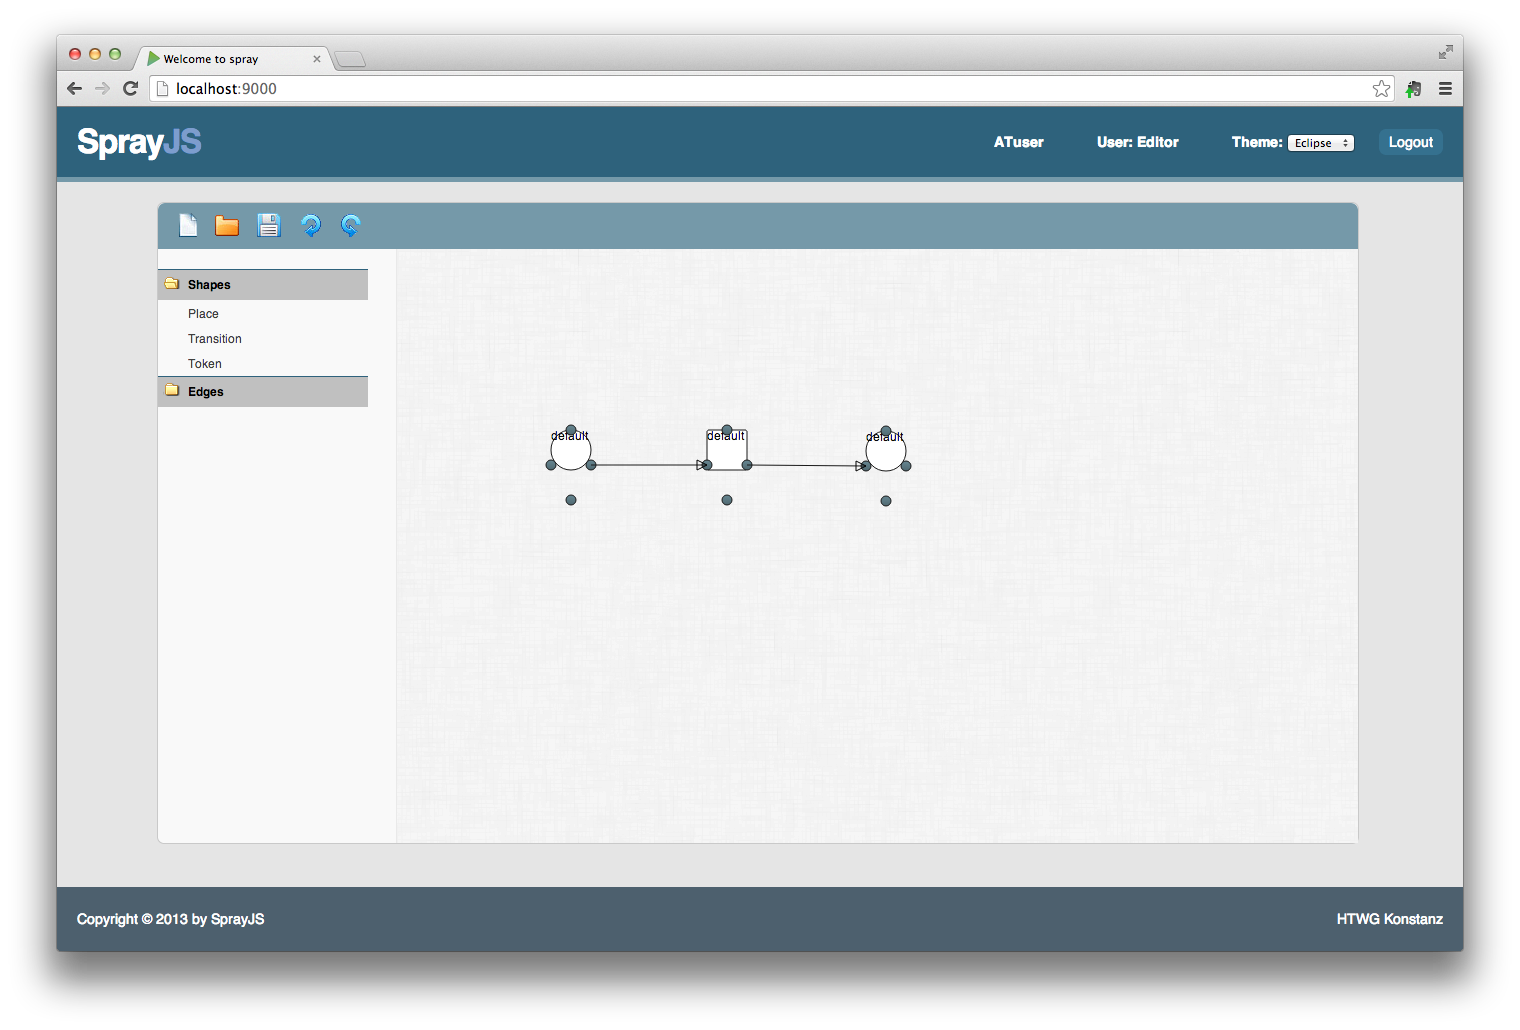
\includegraphics[width=1.0\textwidth]{Figures/Screenshot.png}
  \caption{Screenshot vom gegenwärtigen Stand von Spray Web mit geladenem Petrinetz.}\label{fig.screenshot}
\end{figure}

\subsection{Shapes zeichnen}

Es ist essentiell, dass die Basisshapes gezeichnet werden können.
Zudem sollen die Basisshapes die in Kapitel \ref{sec.primitivShapes}
beschrieben sind, auch ineinander verschachtelbar sein.
Da die Shapes auch u.a. Textfelder enthalten können, um z.B. das Shape
zu benennen, ist es nötig, dass der Benutzer diese verändern kann auch
innerhalb eines verschachtelten Shapes.
Da die Shapes mit Connections zusammen eine Graphenstruktur bilden,
müssen die Shapes über Connections miteinander verbunden werden können.

Es wäre ideal, wenn ein Toolkit existieren würde, welches all diese
Anforderungen erfüllt. Falls ein solches Toolkit nicht existiert,
müsste selbst eines mit den in Kapitel \ref{sec.funcAnforderung}
gestellten Anforderungen gebaut werden.

\paragraph{SVG oder Canvas?} Für diesen konkreten Anwendungsfall ist
SVG die bessere Wahl, siehe dazu Abbildung \ref{fig.svgVsCanvas}.
Ein Hauptgrund\footnote{Vgl. \url{http://dev.opera.com/articles/view/svg-or-canvas-choosing-between-the-two/}} ist u.a. auch, dass weniger Zeilen Code benötigt werden
als bei Canvas (selbst wenn man auf entsprechende Toolkits zurückgreift)
und direkt Vektorgrafiken produziert werden.

\begin{figure}[h!]
  \centering
  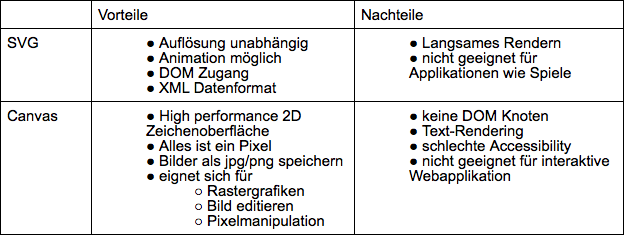
\includegraphics[width=1.0\textwidth]{Figures/Svg_vs_Canvas.png}
  \caption{SVG versus Canvas.}\label{fig.svgVsCanvas}
\end{figure}


\subsubsection{Toolkits}

Folgende Toolkits haben wir auf ihre Tauglichkeit überprüft:

\begin{itemize}
  \item d3.js \\
  Ist ein Toolkit um im Web interaktive Diagramme darzustellen und
  verwendet dabei SVG.
  \item kinetic.js \\
  Ist eine Bibliothek, um eine komfortablere API zu Canvas anzubieten
  und wurde von Simon Schneeberger bereits verwendet.
  \item Raphael.js \\
  Ist ähnlich zu kinetic.js.
  \item LucidCharts \\
  Ist ein Editor ähnlich zu Visio, jedoch im Web mit HTML/CSS/JavaScript,
  setzt auf Canvas.
  \item \dd \\
  Bietet eine ähnliche API wie das aus der Java-Welt bekannte Draw2d,
  es ist in der Lage Shapes und Connections zu zeichnen.
  Verwendet SVG.
  \item go.js \\
  Ist ähnlich zu \dd, jedoch nicht quelloffen.
\end{itemize}

\subsubsection{\dd}

Erst relativ spät haben wir das \dd~Toolkit gefunden.
Es erfüllt quasi alle Anforderungen (siehe Abb. \ref{fig.ddCheck})
und ist damit der Gewinner unter den
durch unsere Recherche untersuchten Toolkits.

\begin{figure}[h!]
  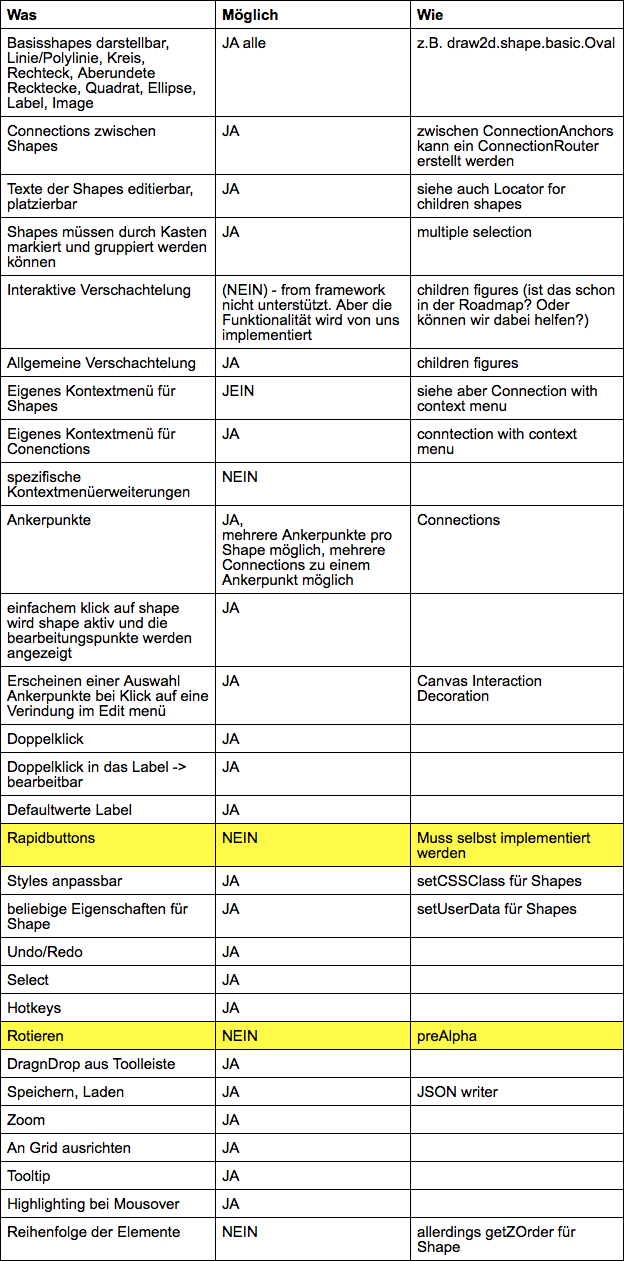
\includegraphics[height=0.9\textheight]{Figures/DD_Anforderungen.png}
  \caption{\dd~Anforderungsüberprüfung.}\label{fig.ddCheck}
\end{figure}

\noindent \dd~wurde von \citep{dd} entwickelt und steht u.a. unter der GNU General
Public Lizenz (GPL) und ist daher auch rein rechtlich geeignet für
das ebenfalls unter einer Open Source Lizenz stehende Spray-Projekt.

\subsubsection{Shape Factory}

Die eigens entwickelte Shape Factory erstellt gemäss der Shape Definition aus Spray das Spray Shape in der Zeichenfläche.
Die Factory kann alle Basis Shapes wie Rectangle, Rounded-Rectangle, Label und weitere als \dd~ Shapes zeichnen.
Sie unterstützt auch die Erzeugung von Anchors. Durch rekursive Iteration der Spray Definition des Shapes wird
das Spray Shape für die Zeichenfläche generisch aufgebaut. So können \dd~ Shapes beliebig ineinander verschachtelt werden.
Als Mutterobjekt des Shapes wird ein Rechteck als Boundingbox verwendet.
Alle weiteren Shapes werden dieser Boundingbox untergeordnet. Jedes so erzeugte Spray Shape erhält eine \dd~ ID und kann somit
für weitere Zwecke angesteuert werden.

\subsubsection{Compartments}

Compartments sind Verschachtelungen einzelner Shapes (oder Gruppen von Shapes).

Draw2d bietet bereits die Möglichkeit zur Verschachtelung von Shapes.
Wenn allerdings Gruppen von Shapes verschachtelt werden sollen, müssen alle Elemente einzeln dem neuen Parent hinzugefügt werden.

Auch die Commands für Undo und Redo mussten implementiert werden.
Dieser Prozess ist etwas aufwändiger weil bereits auf abgeschlossene Commands zugegriffen werden muss. 
Manche Commands we Move werden automatisch erstellt, ausgeführt und auf den CommandStack gelegt.
Insbesondere der Move und Create Command müssen modifiziert/ausgeführt werden.
Hier wurden viele Fälle bereits implementiert.

Beim Laden einer abgespeicherten Zeichenfläche werden Compartments aktuell nur sehr rudimentär unterstützt.

Alternativ kann auch das nur das Laden der Compartments angepasst werden.

Compartments / Verschachtelungen / Komplexe Shapes können durch die Methode
\verb|Canvas.addFigure(child, locator)| erstellt werden.

\begin{verbatim}
var locator = new spray2d.layout.locator.FigureLocator(p);
locator.setPos(p, this.x, this.y);
this.parent.addFigure(this.figure, locator);

// Durch setDraggable(true) kann das hinzugefügt Shape
// eigenständig bewegt werden
this.figure.setDraggable(true);
\end{verbatim}

\subsection{Code-Generierung}

Spray Web ist so aufgebaut, dass es von Spray generierten Code annimmt
und verarbeitet. Da Spray intern um andere Generator-Implementierungen
erweiterbar ist, ist es auch möglich, dass ideal für Spray Web
zugeschnittenen Code erzeugt werden kann.

Die Generatoren sind in Xtend geschrieben, dieses ist wiederum Teil
der Language Workbench
\emph{Xtext}\footnote{Siehe \url{http://www.eclipse.org/Xtext/}}.

Diese Generatoren sind noch nicht ins Spray-Projekt integriert, und müssen
daher noch in die Spray Projektstruktur eingebracht werden.
Man kann den Shape-Generator als Standalone Xtext Projekt zum laufen bekommen,
der Spray-Generator (Logik) muss jedoch in der Eclipse-Umgebung direkt
im Spray-Projekt eingebunden werden, da die Spray-Grammatik nicht ohne
weiteres als Standalone Xtext Projekt extrahiert werden kann.
Um Eclipse Spray (Developer) lauffähig zu bekommen, sind ggf. die fogenden
Links hilfreich:

\begin{itemize}
  \item \url{http://stackoverflow.com/questions/13575695/}
  \item \url{http://stackoverflow.com/questions/17527096/}
  \item \url{http://stackoverflow.com/questions/15374697/}
\end{itemize}

\noindent In der ersten Spray Eclipse-Instanz liegt der eigentliche
Spray-Quellcode. Auf dieser Ebene liegen auch sämtliche Generatoren.
Aus diesem Quellcode kann eine zweite Eclipse-Instanz generiert werden,
in dieser Instanz werden z.B. die Shape- und Spray-Grammatik geschrieben
und Eclipse stößt die entsprechenden Code-Generatoren an um Graphiti-Code
zu generieren -- bzw. für Spray Web: JSON Code.
Dieser Graphiti Code kann wiederum als Eclipse-Instanz ausgeführt werden;
dort ist dann der eigentliche grafische Editor auf Eclipse-Basis -- eben
der gewollte Graphiti Editor.

\subsubsection{Shape Layout Definitionen}

Es soll JSON-Code aus der Shape Grammatik \citep[gemäß][]{sprayUser}
generiert werden. Der Code befindet sich im Repositorium in
{\tt generators/shape\_dsl/ShapeGenerator.xtend}.
Ziel ist es z.B. aus folgender Spray-Shape-Grammatik:

\begin{verbatim}
shape TransitionShape {
  text {
    position (x=0, y=0)
    size (width=30, height=30)
    id = transitionText
  }
  rectangle {
    position(x=0, y=30)
    size (width=40, height=40)  
  }
}
\end{verbatim}

\noindent Ein solches JSON zu generieren:

\begin{verbatim}
{
  name: "TransitionShape",
  params: {
    size: {witdh: 40, height: 70}
  },
  shapes: [
    {
      name: "Text",
      params: {
        size: {width: 30, height: 30},
        align: {
          horizontal: "left",
          vertical: "top"
        }
      }
    },
    {
      name: "Rectangle",
      params: {
        size: {width: 40, height: 40},
      }
    }
  ]
}
\end{verbatim}

\paragraph{JSON Shape Spezifikation}
Komplexe Shapes können aus primitiven Shapes zusammengesetzt werden.
Es gibt folgende primitive Shapes:

\begin{itemize}
  \item Line
  \item PolyLine
  \item Rectangle
  \item RoundedRectangle
  \item Polygon
  \item Ellipse
  \item Text
  \item Anchor
\end{itemize}

\noindent Diese komplexen Shapes werden in einer Datei {\tt genshape.js} in einer
JSON-Datenstruktur abgelegt. Die Datei enthält eine Variable, worin die
Shapes in einer Liste abgespeichert werden:

\begin{verbatim}
var shapedefs = [
  {...},
  {...},
  ...
]
\end{verbatim}

\noindent Jedes \verb|{...}| Objekt entspricht genau einem komplexen Shape.
Jedes dieser Shapes kann folgende Eigenschaften (JSON Properties) besitzen:

\begin{verbatim}
  name    : "..."
  params  : {...}
  anchors : [...]  (only in the top level!)
  shapes  : [...]
\end{verbatim}

\noindent {\tt name} beschreibt entweder das primitive Shape oder wenn es ganz oben
in der Hierarchie steht den Namen des komplexen Shapes.
In {\tt params} können wieder folgende Attribute vorkommen:

\begin{verbatim}
  position : [{x: Int, y: Int, radius: Int, angle: Int, offset: Float}*]
  size : {width: Int, height: Int}
  stretching : {horizontal, vertical}
  align : {horizontal, vertical}
    horizontal : "left" | "center" | "right"
    vertical :  "top" | "middle" | "center"
  curve : {width: Int, height: Int}
  size-min : {width: Int, height: Int}
  size-max : {width: Int, height: Int}
  proportional : Bool
  layout : {stretching | spacing : Int | margin : Int | invisible}
  points : [{x: Int, y: Int, curveBefore: Int, curveAfter: Int}*]
\end{verbatim}

\noindent Nur in der obersten Ebene der Hierarchie können Anker {\tt anchors} definiert werden,
diese betreffen also nur das gesamte komplexe Shape (Anker können also
nicht verschachtelt werden). Es gibt diese Formen von Ankern:

\begin{verbatim}
  {type: "center"}
  {type: "corners"}
  {type: "relative", x: Int, y: Int}
  {type: "fixpoints", x: Int, y: Int}
\end{verbatim}

\noindent Mit der {\tt shapes} Property kann die Verschachtelung des Shapes beschrieben
werden, es darf also die gesamte Shape-Definition hier nochmals (also
rekursiv) vorkommen.

Folgende Parameter dürfen nur in der obersten Ebene der Hierarchie innerhalb
der {\tt params}-Liste vorkommen:

\begin{verbatim}
  minWidth: Int
  minHeight: Int
  maxWidth: Int
  maxHeight: Int
  stretchH: Bool
  stretchV: Bool
  proportional: Bool
\end{verbatim}

\noindent Zudem wird immer für das gesamte komplexe Shape eine Boundingbox berechnet,
d.h. es existiert in der obersten Ebene immer ein {\tt size}-Objekt innerhalb
der {\tt params}.

\paragraph{Compartments} sind spezielle Shapes, die andere Shapes wiederum
zur Laufzeit aufnehmen können. Es können nur Rectangle und Ellipse als
Compartment markiert werden, d.h. sie enthalten innerhalb ihres {\tt params}
Property folgendes Attribut:

\begin{verbatim}
  compartment: {
    locationId: String,
    layout: fixed|vertical|horizontal|fit,
    spacing: Int,
    margin: Int,
    insisible: Bool,
    stretchH: Bool,
    stretchV: Bool
  }
\end{verbatim}

\paragraph{Connections} sind ebenfalls ein Spezialfall von Shape,
welche sich jedoch explizit von den „normalen“ Shapes unterscheiden,
denn sie können nur folgende Eigenschaften besitzen:

\begin{verbatim}
  name: "..."
  connectionType: "freeform" | manhatten
  placings: [ {...}, {...}, ... ]
\end{verbatim}

\noindent Ein \verb|{...}|-Objekt welches in den {\tt placings} vorkommt kann folgende
Attribute enthalten:

\begin{verbatim}
  offset: Double
  distance: Double
  angle: Double
  shape: CDShape
\end{verbatim}

\noindent Ein CDShape ist ein spezielles primitives Shape, welches für Connections
zugelassen ist. Diese kommen auch nur in \emph{nicht} verschachtelter Form vor:

\begin{itemize}
  \item CDLine
  \item CDPolyLine
  \item CDRectangle
  \item CDRoundedRectangle
  \item CDPolygon
  \item CDEllipse
  \item CDText
\end{itemize}


\subsubsection{Spray Logik Definitionen}

Es soll JSON-Code aus der Spray Grammatik generiert werden.
Mit diesen Definitionen kann Spray Web die Benutzereingaben überprüfen,
ob diese zu ein zulässiges Modell führen.
Der Code dazu befindet sich im Repositorium in
{\tt generators/spray\_dsl/SprayJsonGenerator.xtend}.
Ziel ist es z.B. aus folgender Spray-Logik-Grammatik:

\begin{verbatim}
class Place {
  shape PlaceShape {
    name into placeText
    reference tokens into tokensCompartment
  }
  behavior {
    create into mapelements palette "Shapes"
  }
} 
\end{verbatim}

\noindent Solch ein JSON zu generieren:

\begin{verbatim}
{
  name: "Place",
  shape: "PlaceShape",
  compartments: [
    {
      canContain: "Token",
      atLocationId: "tokensCompartment",
    },
  ],
  palette: "Shapes",
}
\end{verbatim}

\paragraph{JSON Spray (Logik) Spezifikation} Die Spray Grammatik definiert
ein Diagramm, welches sich in einzelne Klassen gliedert.
Die Klassen spezifizieren welches Verhalten, welchem Shape zugeordnet wird
bzw. welche Connections zwischen Shapes zulässig sind.

Diese Logik Definitionen werden in einer Datei {\tt genspray.js} abgelegt.
Die Datei enthält eine Variable, worin die einzelnen Klassendefinitionen
in einer Liste gespeichert werden:

\begin{verbatim}
var classdefs = [
  {...},
  {...},
  ...
]
\end{verbatim}

\noindent Es gibt zwei Sorten von \verb|{...}|-Objekten.
Die erste Sorte verbindet Shape und Klasse und kann
folgende Eigenschaften besitzen:

\begin{verbatim}
  name: String
  shape: String
  compartments: [ {...}, ... ]
\end{verbatim}

\noindent Das {\tt compartments} Property enthält die Referenz,
welches Shape in das Compartment gelegt werden darf, sowie das
Shape welches der Compartment-Behälter sein soll:

\begin{verbatim}
  canContain: String
  atLocationId: String
\end{verbatim}

\noindent Die zweite Sorte definiert, welche Klassen mit welchem
Connection-Shape verbunden werden dürfen. Es kann folgende Eigenschaften
besitzen:

\begin{verbatim}
  name: String
  connection: String
  from: String
  to: String
\end{verbatim}

\noindent Wobei {\tt connection} auf das Connectionshape referenziert,
{\tt from} referenziert von welcher Klasse aus die Connection ausgehen darf
und {\tt to} referenziert zu der Klasse zu der die Connection führen darf.

Jede der beiden Sorten muss das {\tt palette} Propterty enthalten.
Dieses definiert, unter welcher Auswahlpalette die Klasse im grafischen Editor
zur Verfügung gestellt wird.

\subsection{Validierung und Persistierung}

Mit dem Spray Framework kann über drei Grammatiken ein grafischer DSL
Editor definiert werden. Mit der Spray Grammatik wird spezifiziert,
wie ein gültiges Modell aussieht.

Der Benutzer des so entstandenen grafischen Editors möchte eine Instanz
dieses Modells erstellen, welche er speichern bzw. laden kann;
zudem sollte vom Editor gewährleistet werden, dass der Benutzer nur
gültige Modelle produzieren kann.

\subsubsection{Validierung im Client}

Der Client erhält die Regeln für ein gültiges Modell im JSON-Format
({\tt classdefs}). Mit diesen Informationen wird die Shape Factory gefüttert
und kann somit schon bei der Erstellung eines Shapes bzw. einer Connection
überprüfen, ob dies eine zulässig Aktion ist.

\subsubsection{Persistierungsverfahren}

In diesem Kapitel werden drei Verfahren diskutiert, mit denen Modellinstanzspeicherung
ermöglicht werden kann.
Ein Verfahren wurde exemplarisch programmiert, da die anderen Verfahren ggf. noch
Mängel aufweisen.

\paragraph{EMF-REST}

\begin{quote}
EMF-REST generates truly RESTful APIs for your EMF models. EMF-REST complements the existing (Java-based) API generation facilities EMF already provides and extends them to the Web.

Thanks to EMF-REST, web developers can quickly get a JSON-based RESTful API derived from their models plus a JavaScript library to simplify the interaction with the API.\footnote{EMF-REST Webseite: \url{http://emf-rest.com/index.html}}
\end{quote}

\noindent EMF-REST stellt ein Eclipse-Plugin bereit, welches aus einem Ecore Metamodell
Quellcodedateien generieren kann, die mit einem Tomcat Server lauffähig sind.
Neben der RESTful API wird auch noch ein passendes JavaScript-Binding generiert.

Bisher kann man jedoch nur eine schon existierende XMI Modellinstanz via
RESTful Abruf \emph{lesen}; das \emph{Schreiben} mit z.B. einem HTTP-PUT
ist noch nicht möglich.

Dazu schrieben wird eine E-Mail an das Entwicklerteam, Camilo Alvarez antwortete:

\begin{quote}
[...] we are implementing the PUT/POST/DELETE methods to complete the API. There will be an option to save the changes in the XMI file.
We plan to release it in february of the next year.
\end{quote}

\noindent Das bedeutet diese wichtigen Funktionen stehen vorr. erst Februar 2014
bereit. Daher haben wir uns vorerst gegen EMF-REST entschieden, auch wenn es
ein sehr vielversprechender Ansatz gewesen wäre.

\paragraph{Ecore.js}

Ecore.js ist eine Ecore (EMOF) Implementierung in JavaScript von Guillaume Hillairet.
Der Quellcode ist verfügbar auf GitHub unter
\url{https://github.com/ghillairet/ecore.js}.
Ecore.js läuft sowohl als JavaScript Clientcode (Browser), als auch als
node.js Servercode.

Der Vorteil hier ist, dass quasi keinerlei Kommunikation zu einem Server nötig ist.
Es ist möglich aus den Ecore Objekten die in JavaScript gehalten werden,
direkt ein XMI oder JSON erstellen zu lassen.
Das würde bedeuten Spray Web könnte komplett autonom, also ohne externe
Abhängigkeiten oder Synchronisierungsprobleme, im Browser arbeiten.
Eine Kollaboration könnte dennoch mit z.B.
Together.js\footnote{\url{https://togetherjs.com/}} erfolgen.

Beispielcode der durch unsere Nachforschungen entstanden ist, wird im Repositorium
unter {\tt archive/ecore\_js} festgehalten.

Schlussendlich haben wir uns dagegen entschieden, da die Kollaboration
über den Server von den Projektauftraggebern bevorzugt wurde und
Ecore für die Java-Platform von einer starken Gemeinschaft gepflegt wird.

\paragraph{Ecore mit Server}
Als Serverlösung wurde ein Web2Ecore-Interface implementiert, welches durch Spray
für jedes Modell automatisiert generiert werden muss. Die Ecore Serverlösung ist mit Reflections weitgehend
dynamisch gehalten. Der Spray Generator muss nur einige wenige Anpassungen hinsichtlich
Modelltyps (z.B. Petrinet) und der Imports der generierten Implementierungsklassen des Ecore Modells vornehmen.

Jede Aktion im Webeditor betreffend Erstellen und Löschen, sei es ein Compartment, Connection oder ein einzelnes Shape, wird
über eine Websocketnachricht dem Web2Ecore-Interface auf dem Server gemeldet. Das Interface verarbeitet die Benachrichtigung
und aktualisiert entsprechend das Ecore-Modell auf dem Server.

Das eigens entwickelte Ecore-Interface unterstützt das Erstellen von Ecore-Objekten auf allen Ebenen.
Wird ein Objekt auf zweiter oder tieferer Ebene erstellt, sprich Compartment, so muss immer das Elternelement
mitangegeben werden. Das Ecore-Interface unterstützt auch die Erstellung von Connections. Dafür muss
bekannt sein welche Connection erstellt werden soll und dessen Start und Zielobjekt.

Ebenso kann das Ecore-Interface Objekte löschen. Alle Fälle sind berücksichtigt: Löschen eines einzelnen Objekts
auf erster Ebene, sowie auf allen nachfolgenden Ebenen (Compartment) und das Löschen von Connections. Wird ebenso 
ein Objekt gelöscht, was als Start oder Zielobjekt einer Connection agiert, so wird auch die Connection aus dem
Ecore-Modell gelöscht.

Damit das erstellte oder gelöschte Shape in der Weboberfläche auch dem Shape im Ecore-Modell entspricht, ist ein Mapping
zwischen den beiden Elementen nötig. Das Mapping erfolgt über einen Index. Jedes Element in der Zeichenfläche besitzt einen Index
welche der Erstellungsreihenfolge entspricht. Bei einem Compartment muss der Index des Elternelements mitangegeben werden. Wird ein Shape
innerhalb eines Shapes erstellt (Compartment) so wird der Index wieder von vorne gezählt, dazu muss zusätzlich der Index ders Elternelements
mitangegeben werden. Das Mapping ist keine triviale Angelegenheit und muss optimiert werden. Die Berechnung des Index kann unter
Umständen unnötig viel Rechenzeit beanspruchen.

Da nur valide Modelle in Spray Web gezeichnet werden können, ist auch das Ecore-Modell stets valide.
Das Ecore-Modell wird als XMI-Dokument abgespeichert und enthält lediglich die Objekte ohne
Eigenschaften zur Zeichenfläche. Die Zeichenfläche wird in JSON festgehalten und beinhaltet alle Informationen
die der User selbst ändern kann. Das umfasst die Position der Elemente, deren Skalierung, das Label und über welche Anker
welche Connection gesetzt sind. Die Speicherung der Compartments sind an dieser Stelle
noch nicht implementiert worden. Die Zeichenfläche muss zusätzlich zum Ecore-Modell auf dem Server persistiert werden.
Die Persistierung der Zeichenfläche muss bei jeder Benutzeraktion erfolgen, die auch eine Aktualisierung des Ecore-Modells
bewirkt. Wenn der Web Editor neu geladen wird, so muss der letzte Zustand der Zeichenfläche vom Server an den Client
gesendet, im Editor geladen und somit dargestellt werden. Ansonsten würde der Benutzer beim Neuladen des Editors
mit einer leeren Zeichenfläche starten, das zugrundeliegende Ecore-Modell ist aber in einem anderen Zustand.
So wäre das Ecore-Modell nicht mehr mit der Zeichenfläche konsistent. Zukünftig muss an dieser Stelle
eine sinnvolle Synchronisierung implementiert werden, so dass Ecore-Modell und Zeichenfläche auf dem Server zu jedem Zeitpunkt
konsistent sind.

In Spray Web wird die Zeichenfläche erst beim expliziten Speichern (Klick auf das Speichern-Icon) auf dem Server persisistiert.
Unter Umständen kann es aber sein, dass der Benutzer nach dem Speichern noch Aktionen tätigt, die das Ecore-Modell aktualisiert.
Wenn der Benutzer nun die Zeichenfläche neu lädt, so stimmt sie nicht mehr mit Ecore-Modell überein.

Durch die umgesetzte Web2Ecore-Lösung bleibt das Ecore-Modell stets auf dem Server aktuell. Damit ist ein wesentlicher Baustein
für Multikollaboration gesetzt. Jeder Benutzer der mit derselben Zeichenfläche arbeitet, verwendet so auch das gleiche
zugrunde liegende Ecore-Modell.

\subsection{Änderungen am Framework (Patches)}

\dd~ deckt nicht alle Funktionen ab um die benötigten Anforderungen an Spray Web zu erfüllen.
Aus dem Grund musste das \dd~ Framwork an einigen Stellen erweitert werden.
So weit es das Framwork zugelassen hat, wurden Klassen abgeleitet um das Framework so wenig wie möglich unverändert zu lassen.
Somit kann das Framework problemlos aktualisiert werden.

An einigen Stellen ist komponentengetrenntes Entwickeln nicht realisierbar, da abstrakte Klassen auch
implementierte Methoden besitzen und JavaScript keine vollständige objekt-orientierte Programmierung unterstützt. 
Unter Umständen hätten ganze Vererbungshierarchien abgeleitet werden müssen um Basis-Funktionalität vom Framework
getrennt zu erweiteren.

Die Differenz von der Originalversion 3.0.0 und den Änderungen von uns kann mit dem Befehl 
{\tt git diff 57a7d13 -- sprayServer/public/javascripts/spray/lib/draw2d\_3.0.0/src}
ermittelt und visualisiert werden.
